\chapter{Software Quality}

\begin{center}
  \begin{minipage}{0.65\linewidth}

    ISO/IEC 9126: issued in 1991 and revised in 2001, being retired.
    Iso/IEC 25XX - SQuaRE: Software Product Quality Requirements and Evaluation.
    Is a family of standards in development.
  \end{minipage}%
  \hfill
  \begin{minipage}{0.3\linewidth}
    \centering
    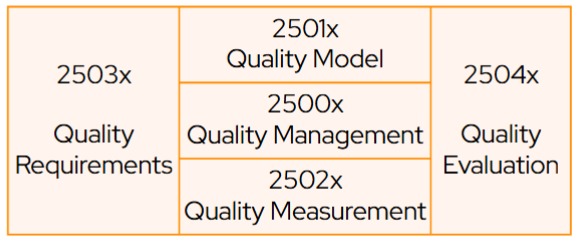
\includegraphics[width=\linewidth]{content/chapters/images/2026-05-09-15-09-16.png}
  \end{minipage}
\end{center}

Software quality is divided in two parts: Product quality (internal,
external, in use, data) and process quality.

\begin{figure}[h!]
  \centering
  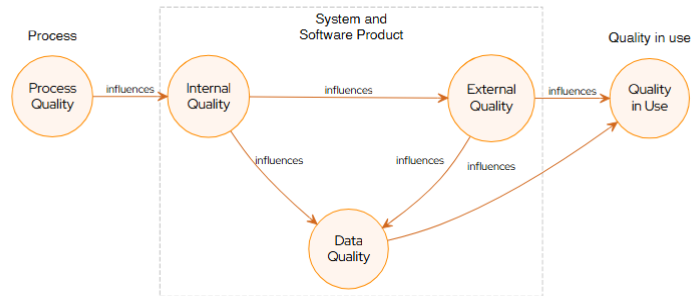
\includegraphics[width=\linewidth]{content/chapters/images/2026-05-09-15-12-00.png}
\end{figure}

\section{Target entities}
Product quality addresses several different entities in a
complex information system

\begin{figure}[h!]
  \centering
  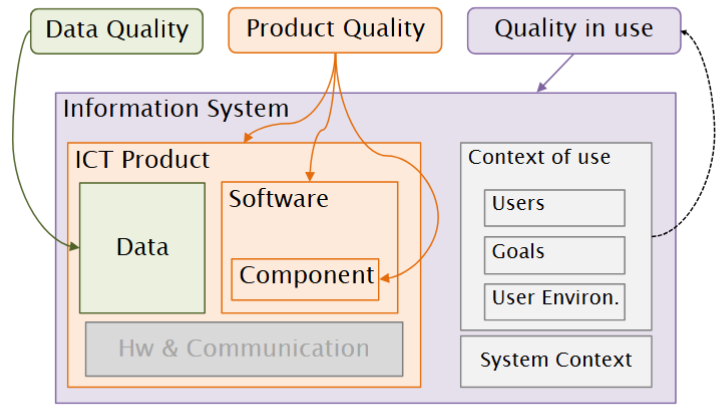
\includegraphics[width=\linewidth]{content/chapters/images/2026-05-09-15-12-58.png}
\end{figure}

\subsection{Model structure}

\begin{itemize}
  \item \textbf{Characteristics}: main aspects eg. usability
  \item \textbf{Sub-characteristics}: specific aspects eg. accessibility
  \item \textbf{Metrics}: evaluate a specific (sub)-characteristic, eg. number of clicks to reach a page
  \item \textbf{Measure elements}: Fundamental
\end{itemize}

\section{Software product quality}

\begin{itemize}
  \item Functional suitability
  \item Performance efficiency
  \item Compatibility
  \item Interaction capability (Usability)
  \item Reliability
  \item Security
  \item Maintainability
  \item Flexibility
\end{itemize}

\subsection{Functional suitability}

Capability of a product to provide functions that meet stated
and implied needs of intended users when it is used under
specified conditions: completeness, correctness, appropriateness.

\subsection{Performance efficiency}

Capability of a product to perform its functions within specified
parameters and be efficient in the use of resources under
stated condition: time behaviour, resource utilization, capacity.

\subsection{Compatibility}
Capability of a product or its component to exchange
information with other products, systems or components, and/
or perform its required functions, while sharing the same
hardware or software environment: co-existence, interoperability.

\subsection{Interaction capability (Usability)}
Capability of a product to be used by specified users to achieve
specified goals with effectiveness, efficiency and satisfaction in
a specified context of use: Recognizability, learnability, operability.

\subsection{Reliability}
Capability a product, to perform specified functions under
specified conditions for a specified period of time: maturity, availability, fault tolerance, recoverability.

\subsection{Security}
Capability of a product to protect information and data so that
persons or other products or systems have the degree of data
access appropriate to their types and levels of authorization,
and to defend against attack patterns by malicious actors: confidentiality, integrity.

\subsection{Maintainability}
Capability of a product to be modified by the intended
maintainers with effectiveness and efficiency: modularity, reusability, analysability, modifiability, testability.

\subsection{Flexibility}
Capability of a product to serve a different or expanded set of
requirements or contexts of use; or the ease with which the
product can adapt itself to changes in its requirements,
contexts of use, or system environment: adaptability, installability, replaceability.

\subsection{Sub-characteristics}

\begin{center}
  \begin{minipage}{0.47\linewidth}
    \centering
    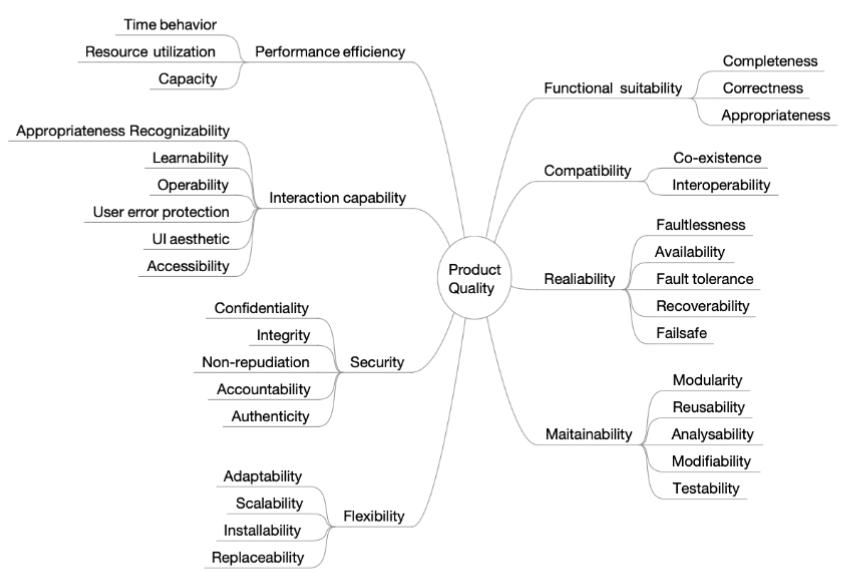
\includegraphics[width=\linewidth]{content/chapters/images/2026-05-09-15-25-16.png}
  \end{minipage}%
  \hfill
  \begin{minipage}{0.47\linewidth}
    \centering
    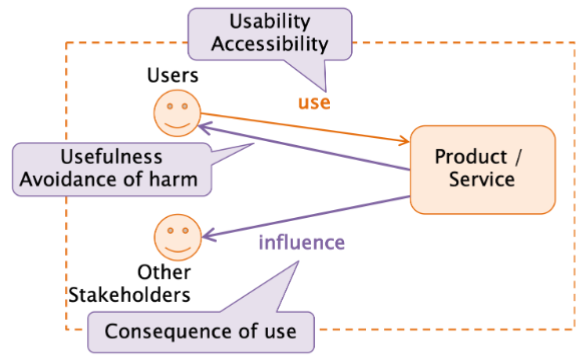
\includegraphics[width=\linewidth]{content/chapters/images/2026-05-09-15-53-18.png}
  \end{minipage}
\end{center}


\subsection{Usability - User error protection}

\begin{table}[h!]
  \renewcommand{\arraystretch}{1.6}
  \centering
  \begin{tabularx}{0.75\textwidth}{X X}
    \toprule
    \textbf{ID}          & \textbf{UEp-1-G}                                                                                                                                     \\
    \midrule
    Name                 & Avoidance of user operation error                                                                                                                    \\
    Description          & What portion of user actions and inputs are protected against causing any system malfunction?                                                        \\
    Measurement function & X = A/B, where A = # user actions and inputs protected against causing any system malfunction; B = # user actions and inputs that could be protected \\
    Interpretation       & $0 \leq X \leq 1$ The closer to 1 the better                                                                                                         \\
    \bottomrule
  \end{tabularx}
\end{table}

\subsection{Reliability - Maturity}

\begin{table}[h!]
  \renewcommand{\arraystretch}{1.6}
  \centering
  \begin{tabularx}{0.75\textwidth}{X X}
    \toprule
    \textbf{ID}          & \textbf{RMa-1-G}                                                                                                                                           \\
    \midrule
    Name                 & Test coverage                                                                                                                                              \\
    Description          & How much of the required test cases has been executed during testing?                                                                                      \\
    Measurement function & X = A/B, where A = #  test cases actually performed representing operation scenario during testing; B = # test cases to be performed to cover requirements \\
    Interpretation       & $0 \leq X \leq 1$ The closer to 1 the better                                                                                                               \\
    \bottomrule
  \end{tabularx}
\end{table}

\subsection{Maintainability - Modularity}

\begin{table}[h!]
  \renewcommand{\arraystretch}{1.6}
  \centering
  \begin{tabularx}{0.75\textwidth}{X X}
    \toprule
    \textbf{ID}          & \textbf{MMo-2-S}                                                                                                                                                                                                                                                             \\
    \midrule
    Name                 & Cyclomatic Complexity                                                                                                                                                                                                                                                        \\
    Description          & How many software modules have the acceptable cyclomatic complexity?                                                                                                                                                                                                         \\
    Measurement function & X = A/B, where A = #  of software modules which have the cyclomatic complexity exceeds a threshold; B = # of software modules in a product. Threshold is defined by each project or organization and is possibly different value by a programming language, or type of module \\
    Interpretation       & $0 \leq X \leq 1$ The closer to 1 the better                                                                                                                                                                                                                                 \\
    \bottomrule
  \end{tabularx}
\end{table}


\section{Quality in Use}

\begin{figure}[h!]
  \centering
  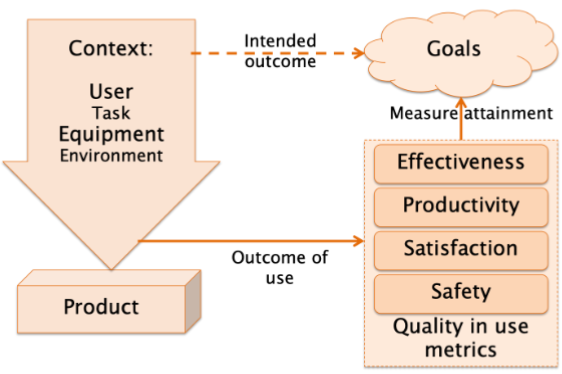
\includegraphics[width=0.5\linewidth]{content/chapters/images/2026-05-09-15-45-47.png}
\end{figure}

\subsection{Quality in Use - Characteristics}

\begin{itemize}
  \item Effectiveness: accuracy and completeness with which identified goals
        are achieved
  \item Efficiency: resources used in relation to the results achieved
  \item Satisfaction: extent to which a user or other stakeholder perceives
        the results of use of a system, product or service to meet their needs and
        expectations
  \item Freedom from risk: degree to which the quality of a product or system
        mitigates or avoids potential risk to the user, organisation or project,
        including risks to economic status, human life, health, or the environment.
  \item Context coverage: degree to which a product or system can be used with
        effectiveness, efficiency, satisfaction, and freedom from risk in both specified
        contexts of use and in contexts beyond those initially explicitly identified.
\end{itemize}

\subsection{Maintainability - Effectiveness}

\begin{table}[h!]
  \renewcommand{\arraystretch}{1.6}
  \centering
  \begin{tabularx}{0.75\textwidth}{X X}
    \toprule
    \textbf{ID}           & \textbf{MMo-2-S}                                                                                                     \\
    \midrule
    Purpose               & Cyclomatic Complexity                                                                                                \\
    Method of application & How many software modules have the acceptable cyclomatic complexity?                                                 \\
    Definition            & $M1 = | 1 - \sum A_i|$, where $A_i$ = # Proportional value of each missing or incorrect component in the task output \\
    Interpretation        & $0 \leq M1 \leq 1$ The closer to 1 the better                                                                        \\
    \bottomrule
  \end{tabularx}
\end{table}

\subsection{Quality in Use Influences}
\begin{itemize}
  \item Influence by use: usability and accessibility
  \item Influence by use of output: Perceived usefullness and Avoidance of harm
  \item Influence of context: Consequence of use
  \item Context coverage: Context completenss and Context extensibility
\end{itemize}


\section{Data quality}
Characteristics from two perspectives:

\begin{itemize}
  \item \textbf{Inherent}: Focus on the data itself, their structure, schema, and semantics
  \item \textbf{System dependent}: Focus on how the data is stored and processed
\end{itemize}

\begin{table}[h!]
  \renewcommand{\arraystretch}{1.6}
  \centering
  \begin{tabular}{l c c}
    \toprule
    \textbf{Inherent} & \textbf{Inher. / Sys. Dep.} & \textbf{Sys. Dep.} \\
    \midrule
    Accuracy          & Accessibility               & Availability       \\
    Completeness      & Compliance                  & Portability        \\
    Consistency       & Confidentiality             & Recoverability     \\
    Currency          & Efficiency                  &                    \\
    Credibility       & Precision                   &                    \\
                      & Understandability           &                    \\
                      & Traceability                &                    \\
    \bottomrule
  \end{tabular}
\end{table}

\subsection{Accuracy}

Correspondence between data and reality

\begin{itemize}
  \item \textbf{Syntactic}: Value belongs to a set of validated information
  \item \textbf{Semantic}: The meaning, the content, corresponds to the reality
\end{itemize}

\subsubsection{Accuracy: Open vs. Closed world}


\begin{itemize}
  \item Closed World Assumption (CWA): The knowledge represented in the data (and its schema) is
        complete. E.g., if a code appears in the list of valid codes it is
        accurate, otherwise it is wrong.
  \item Open World Assumption (OWA): The knowledge about the data is (knowingly) incomplete E.g., if a code is in the list of valid ones it is accurate,
        otherwise it is not possible to immediately decide
\end{itemize}









